%%%%%%%%%%%%%%%%%%%%%%%%%%%%%%%%%%%%%%%%%
% Beamer Presentation
% LaTeX Template
% Version 1.0 (10/11/12)
%
% This template has been downloaded from:
% http://www.LaTeXTemplates.com
%
% License:
% CC BY-NC-SA 3.0 (http://creativecommons.org/licenses/by-nc-sa/3.0/)
%
%%%%%%%%%%%%%%%%%%%%%%%%%%%%%%%%%%%%%%%%%

%----------------------------------------------------------------------------------------
%	PACKAGES AND THEMES
%----------------------------------------------------------------------------------------

\documentclass{beamer}

\mode<presentation> {

\usetheme{Madrid}

\setbeamertemplate{navigation symbols}{} % To remove the navigation symbols from the bottom of all slides uncomment this line
}

\usepackage{graphicx} % Allows including images
\usepackage{booktabs} % Allows the use of \toprule, \midrule and \bottomrule in tables
\usepackage{amssymb}
\usepackage{amsmath}
\usepackage{textpos}
\usepackage{subfigure}
\usepackage{cite}
\usepackage[T1]{fontenc}

\usepackage{listings}


\definecolor{gray}{rgb}{0.4,0.4,0.4}
\definecolor{darkblue}{rgb}{0.0,0.0,0.6}
\definecolor{cyan}{rgb}{0.0,0.6,0.6}

\lstset{
  basicstyle=\ttfamily,
  columns=fullflexible,
  showstringspaces=false,
  commentstyle=\color{gray}\upshape
numbers=right, 
                numberstyle=\tiny, 
                breaklines=true,
                numbersep=5pt,
                xleftmargin=.25in,
                xrightmargin=.25in
}

\lstdefinelanguage{XML}
{
  morestring=[b]",
  morestring=[s]{>}{<},
  morecomment=[s]{<?}{?>},
  stringstyle=\color{black},
  identifierstyle=\color{darkblue},
  keywordstyle=\color{cyan},
  morekeywords={xmlns,version,type}% list your attributes here
}

\DeclareMathOperator*{\argmax}{\arg\!\max}

\title[Automatic Metadata Extraction]{Automatic Metadata Extraction with Conditional Random Fields} % The short title appears at the bottom of every slide, the full title is only on the title page

\author{Joseph Boyd} % Your name
\institute[EPFL] % Your institution as it will appear on the bottom of every slide, may be shorthand to save space
{
\'Ecole Polytechnique F\'eq\'erale de Lausanne \\ % Your institution for the title page
\medskip
\textit{joseph.boyd@epfl.ch} % Your email address
}
\date{\today} % Date, can be changed to a custom date

\begin{document}

\begin{frame}
\titlepage % Print the title page as the first slide
\end{frame}

%------------------------------------------------

\section{The Problem}
\begin{frame}[noframenumbering]{Outline}
\tableofcontents[currentsection, currentsubsection]
\end{frame}

%------------------------------------------------

\begin{frame}
\frametitle{The Problem}
\begin{itemize}
\item Metadata extraction of scientific articles is a well-studied problem
\item Metadata usually refers to header information (title, authors, publisher, abstract...), bibliographic information (citations and their sub-components), document structure (sections, etc.)
\item Extraction of metadata refers to processing and then \emph{classifying} text blocks and other components of the document.
\item The problem is difficult because of the wide variety of document formats that may appear
\end{itemize}
\end{frame}

\begin{frame}
\frametitle{The Problem - An Illustration}
\begin{figure}[!t]
\center
\subfigure{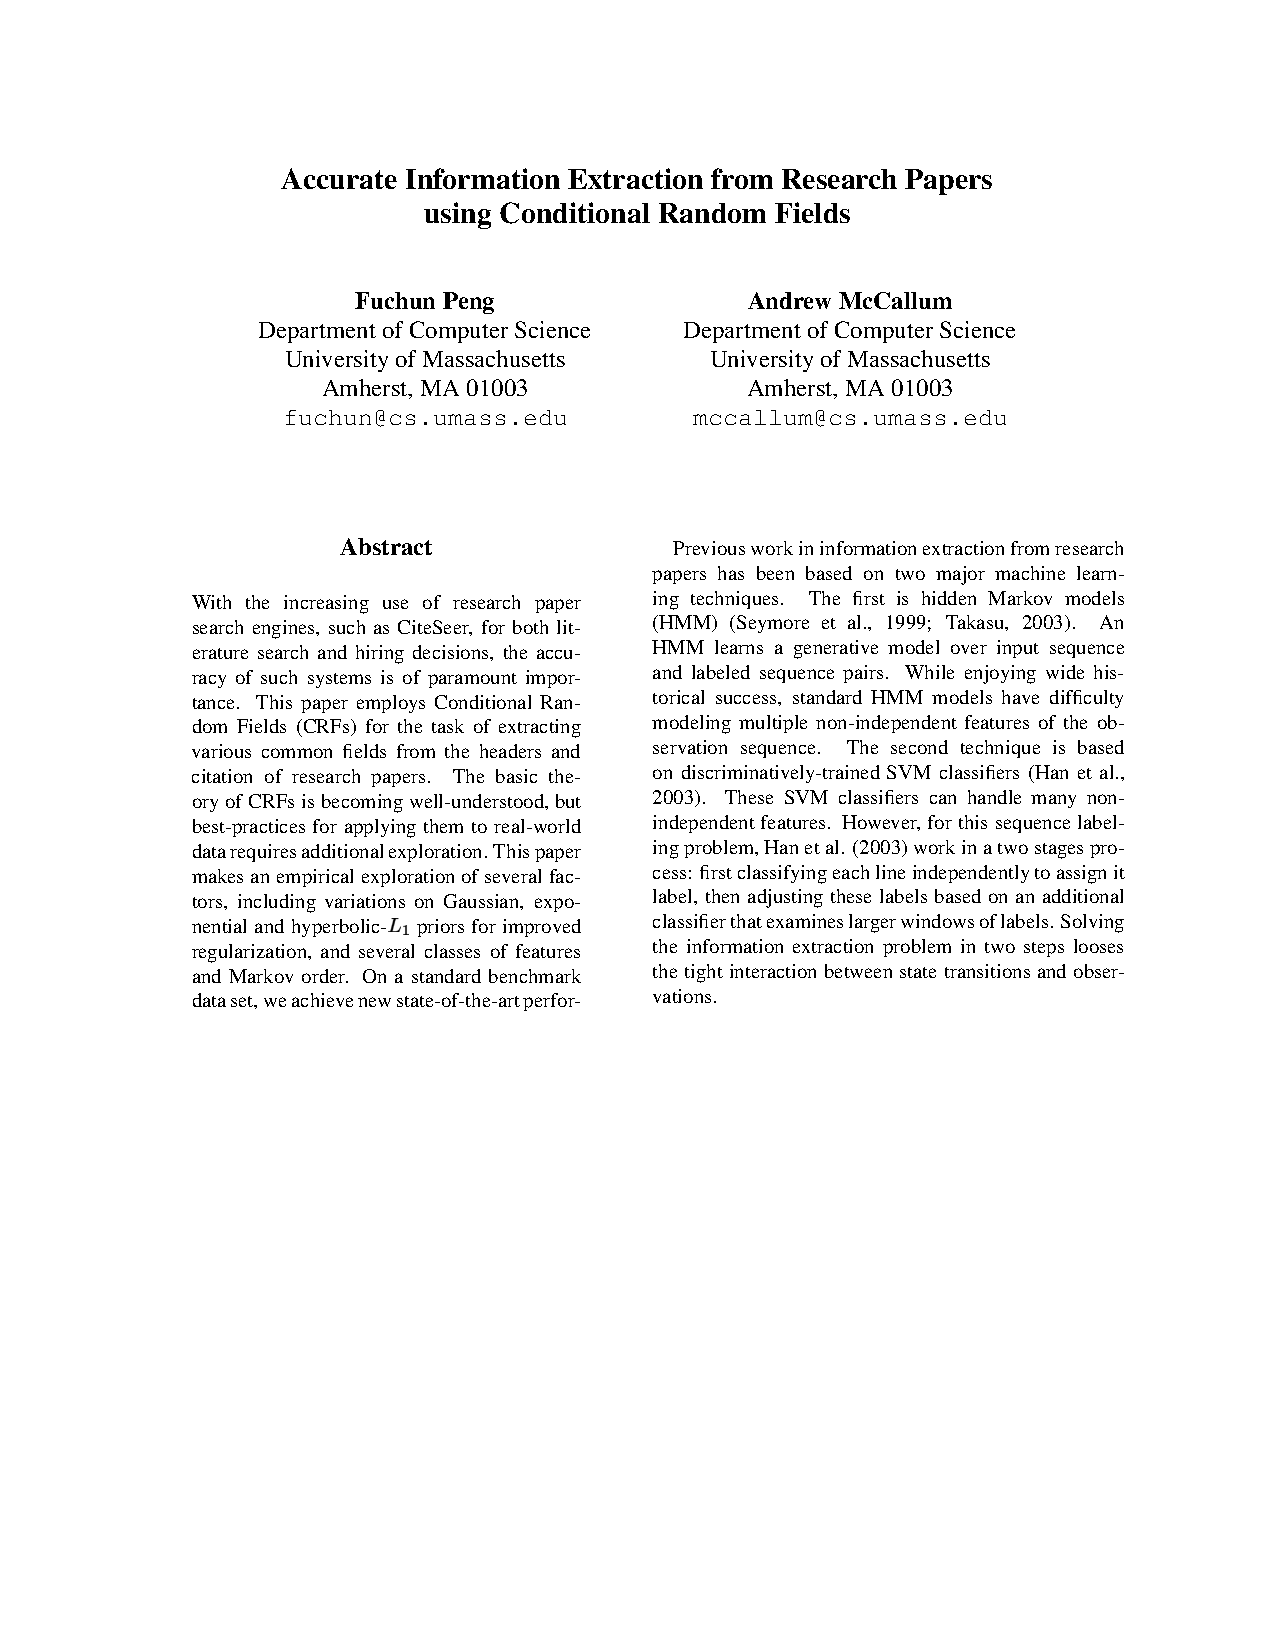
\includegraphics[width=2.25in]{figures/header1.pdf} \label{fig:predictionerror}}
%\hfill
%\subfigure{\raisebox{19mm}{\includegraphics[width=0.5in]{Figures/plus.png} \label{fig:predictionerror}}}
%\hfill
\subfigure{
\includegraphics[width=2.25in]{figures/header2.pdf} \label{fig:logvsrand}}
\end{figure}
\end{frame}

%------------------------------------------------

\begin{frame}
\frametitle{The Problem - Some Assumptions}
\begin{itemize}
\item We are always dealing with PDF documents, and an OCR tool gives us access to the plaintext and OCR information (font, size, orientation,...).
\item Metadata has structure and is not completely random, but it is infeasible to model deterministically $\Rightarrow$ the task is inherently error-prone.
\item There is no one-size-fits-all model for processing a full document $\Rightarrow$ the problem must be decomposed.
\end{itemize}
\end{frame}

%------------------------------------------------

\begin{frame}
\frametitle{The Problem - Solutions}
There are a number of approaches to metadata extraction:
\begin{itemize}
\item Template-based
\item Knowledge base (consult online repositories)
\item Machine learning techniques (HMMs, SVMs, CRFs)
\end{itemize}
In practice, tools for metadata extraction combine these approaches (an example of which we will see later). % \cite{comparison}
\end{frame}

%------------------------------------------------

\section{Theory}
\subsection{Hidden Markov Models}

%------------------------------------------------

\begin{frame}[noframenumbering]{Outline}
\tableofcontents[currentsubsection]
\end{frame}

%------------------------------------------------

\begin{frame}
\frametitle{Hidden Markov Models (HMMs)}
\begin{itemize}
\item Hidden Markov Models (HMM) form a probabilistic model on sequential data.
\item We have a sequence of observations, and we want to predict the ``hidden'' states which generate them.
\item The Markov condition postulates a dependence of one state to the next as we move in time.
\item HMMs have applications in fields as diverse as text processing, bioinformatics, and artificial intelligence.
\end{itemize}
\end{frame}

%------------------------------------------------

\begin{frame}
A well-known application of HMMs is from Natural Language Processing (NLP) - Part of Speech (PoS) tagging.
\frametitle{Hidden Markov Models (HMMs) - Example}
\begin{figure}[!ht]
\center
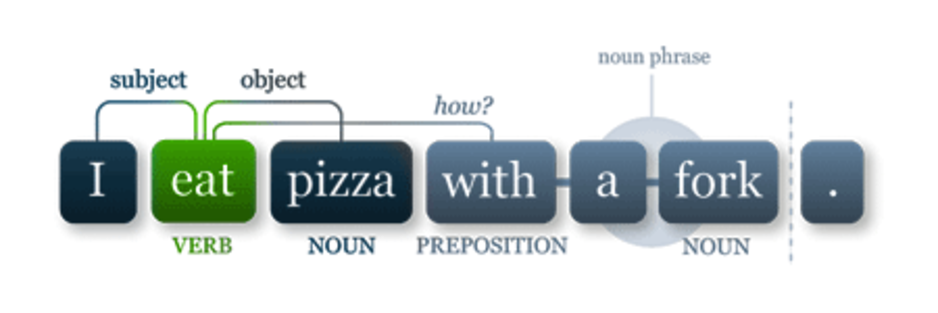
\includegraphics[width=3in]{figures/pos1.pdf}
\end{figure}

\begin{figure}[!ht]
\center
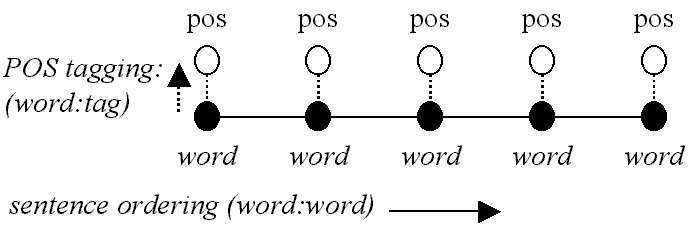
\includegraphics[width=3in]{figures/pos2.png}
\end{figure}
Metadata extraction is a similar problem...
\end{frame}

%------------------------------------------------

\begin{frame}
\frametitle{Hidden Markov Models (HMMs) - Prediction}
\begin{itemize}
\item A Hidden Markov Model factorises in the following way:
$$p(\mathbf{x}, \mathbf{y}) = \prod_{t=1}^T p(y_t | y_{t-1})p(x_t | y_t)$$
\item The probabilities $p(y_t | y_{t-1})$ are ``transition'' probabilities, and $p(x_t | y_t) $``emission'' probabilities, and must be calculated in advance.
\item When it comes to prediction, we use dynamic programming Viterbi algorithm ($\mathcal{O}(T|S|^2))$ to maximise the conditional distribution:
$$\textbf{y}_{prediction} = \argmax_{\textbf{y}} p(\textbf{y} | \textbf{x}) = \argmax_{\textbf{y}}\Bigg\{\prod_{t=1}^T p(y_t | y_{t-1})p(x_t | y_t)\Bigg\}$$
\end{itemize}
Take home message: we can (efficiently) predict the hidden sequence by maximising a likelihood.
\end{frame}

%------------------------------------------------

\subsection{Logistic Regression}

%------------------------------------------------

\begin{frame}[noframenumbering]{Outline}
\tableofcontents[currentsubsection]
\end{frame}

%------------------------------------------------

\begin{frame}
\frametitle{Logistic Regression}
\begin{itemize}
\item A logistic regression is used for classifying a data sample into two (binary) or more (multi) categories, thus,
$$\hat{\text{y}}_{prediction} = \sigma\big(\boldsymbol\beta^{T} \cdot \boldsymbol{x}_{sample}\big),$$
where $\hat{y}$ is the prediction (represented as a probability), $\boldsymbol{x} = [x_0, x_1, ..., x_D]^T$ is a data sample, and $\boldsymbol\beta = [\beta_0, \beta_1, ..., \beta_D]^T$ is the vector of parameters we must \emph{learn}
\item We construct a (maximum log likelihood) cost function in terms of this parameter vector,
$$\mathcal{L}(\boldsymbol\beta) = \sum_{n=1}^N y_n\boldsymbol\beta^T\boldsymbol{x}_n - \log[1 + \exp(\boldsymbol\beta^T\boldsymbol{x}_n)]$$
\end{itemize}
\end{frame}

%------------------------------------------------

\begin{frame}
\frametitle{Solving a Logistic Regression}\begin{itemize}
\item Building a regression model is equivalent to solving a convex optimisation problem (i.e. minimising the cost function)
\item We know the form of the model, and we have a set of (training) data
\item We want to choose the model parameters for which the error is minimised (think line of best fit)
\item We use a numerical method to find the global minimum of error, for example, the method of gradient descent:
$$\boldsymbol\beta^{k+1} = \boldsymbol\beta^{k} - \alpha\nabla\mathcal{L}(\boldsymbol\beta^{k})$$
\end{itemize}
Take home message: we can automatically build mathematical functions for making predictions.
\end{frame}

%------------------------------------------------

\subsection{Conditional Random Fields}

%------------------------------------------------

\begin{frame}[noframenumbering]{Outline}
\tableofcontents[currentsubsection]
\end{frame}

%------------------------------------------------

\begin{frame}
\frametitle{Conditional Random Fields (CRFs)}
\begin{itemize}
\item CRFs belong with HMMs to a class of models called \emph{graphical} models.
\item Classifiers such as logistic regression only predict a single class; graphical models predict a full sequence.
\item CRFs learn paramaters like logistic regression, unlike HMMs where they are precomputed.
\item Modelling the conditional probability, $p(\textbf{y} | \textbf{x})$ is sufficient for classification, so a CRF avoids modelling the distribution on $\textbf{x}$, while allowing a freer choice of features (expressed as feature functions).
\item Whereas with a HMM we model an observation's \emph{occurrence}, with a CRF we can  model richer information about an observation.
\end{itemize}
\end{frame}

% ------------------------------------------------

\begin{frame}

\frametitle{Conditional Random Fields (CRFs)}
\begin{itemize}
\item A conditional random field factorises as,
$$p(\textbf{y}|\textbf{x}) = \frac{p(\textbf{x}, \textbf{y})}{\sum_{y'}{p(\textbf{x}, \textbf{y}')}},$$ where
$$
p(\textbf{x}, \textbf{y}) = \text{exp} \Bigg\{
\sum_{i \in S}
\sum_{j \in S}
\lambda_{ij}
F_{ij}(\textbf{y})
+ 
\sum_{i \in S}
\sum_{o \in O}
\mu_{io}
F_{io}(\textbf{x}, \textbf{y})
\Bigg\}.
$$
Choosing $F_{io}(\textbf{x}, \textbf{y}) \approx \text{feature engineering}$
\end{itemize}

\end{frame}


%IT'S ALL VERY WELL FOR HMMS WHICH DROP THE P(X) ANYWAY WHEN IT COMES TO PREDICTION, BUT THIS IS NO GOOD FOR TRAINING A CLASSIFIER. AND SO WE DIVIDE THROUGH WITH THE P(X) AND FACTOR IT OUT IMPLICITLY BY THE LAW OF TOTAL PROBABILITIES. THIS IS THE TRICK OF CONDITIONAL RANDOM FIELDS.

% ------------------------------------------------

\begin{frame}
\frametitle{Conditional Random Fields (CRFs)}
\begin{itemize}
\item Like a logistic regression we have a cost function to minimise using greatest ascent techniques and solve for model parameters.
\item And the optimisation algorithm is usually an approximation (l-BFGS).
\item There are some further tricks during training (inference algorithms).
\item Prediction is (as with HMMs) done using the Viterbi algorithm, since our factorisation is a function of both observations ($\mathbf{x}$) and states ($\mathbf{y}$).
\end{itemize}
Take home message: CRFs are very similar to HMMs: we predict in the same way, but we learn parameters through training. Modelling the conditional distribution gives us the freedom to exploit richer features.
\end{frame}

% ------------------------------------------------

\section{Grobid}
\begin{frame}[noframenumbering]{Outline}
\tableofcontents[currentsection]
\end{frame}

%------------------------------------------------

\begin{frame}
\frametitle{Grobid}
\begin{itemize}
\item Grobid (GeneRation Of BIbliographic Data) is a Java-based tool for managing CRF models for metadata extraction.
\item It coordinates the training and usage of a ``cascade'' of models, computed with a CRF engine backend.
\item It may also query the web service ``CrossRef'' for verification.
\end{itemize}
\begin{figure}[!ht]
\center
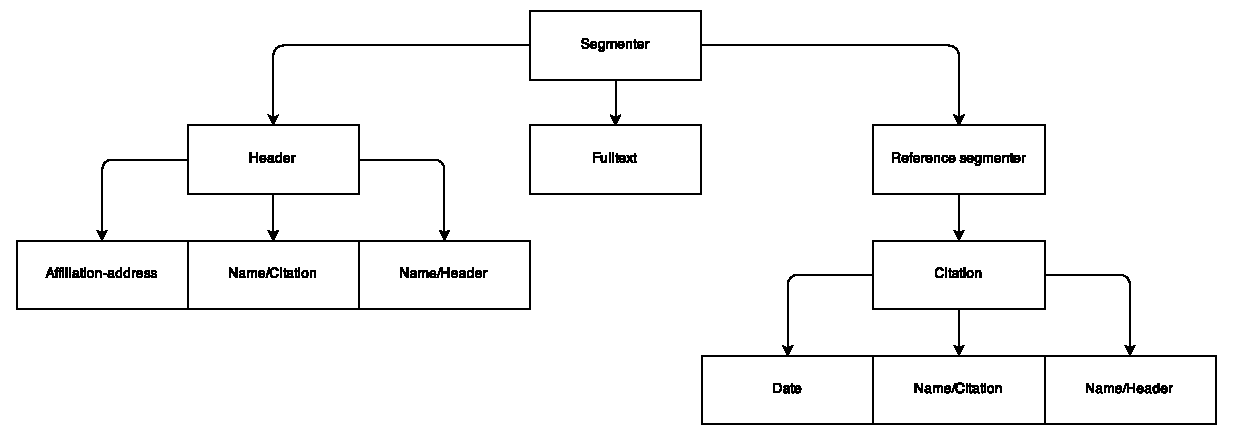
\includegraphics[width=3.75in]{figures/cascade.pdf}
\caption{Cascade of models used by Grobid}
\end{figure}
\end{frame}

%------------------------------------------------

\begin{frame}[fragile]
\frametitle{Grobid - Details}

\begin{figure}
\lstset{language=XML}
\begin{lstlisting}
<bibl>
	<author>V. Gundelach and D. Eisenburger</author>, \&quot; 
	<title level="a">Principle of a direction sensitive borehole antenna with advanced technology and data examples</title>, \&quot; in 
	<title level="m">Proceedings of the 4th International Workshop on Advanced Ground Penetrating Radar (IWAGPR \&apos;07)</title>, pp. 
	<biblScope type="pp">28–31</biblScope>, 
	<date>June 2007</date>.
</bibl>
\end{lstlisting}
\caption{Sample tagged citation for Grobid training input.}
\end{figure}

\end{frame}

%------------------------------------------------

\begin{frame}
\frametitle{Grobid - Training and Prediction}
\begin{figure}[!ht]
\center
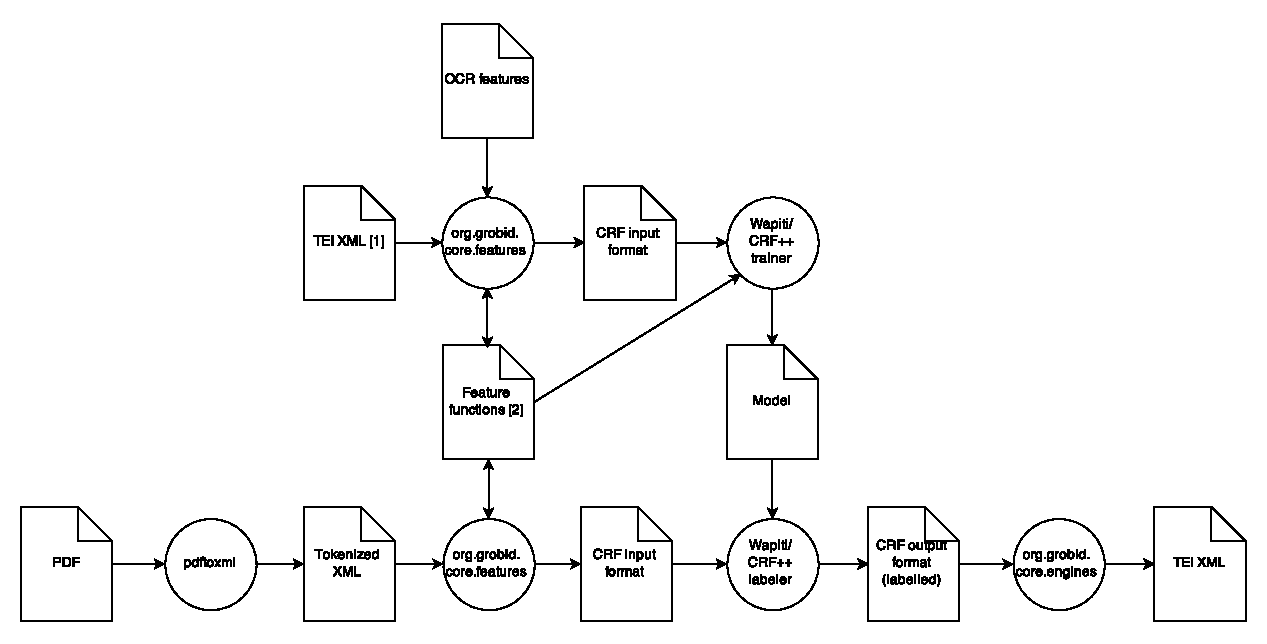
\includegraphics[width=4.5in]{figures/grobid.pdf}
\caption{Training and prediction with Grobid}
\end{figure}
\end{frame}

%------------------------------------------------

\section{Initial Results}
\begin{frame}[noframenumbering]{Outline}
\tableofcontents[currentsection]
\end{frame}

%------------------------------------------------

\begin{frame}
\frametitle{Initial Results - Reference Segmentation}
\begin{center}
\begingroup

\fontsize{8pt}{10pt}\selectfont
\begin{table}[h]
\begin{tabular}{ccccc}
\hline
label		&accuracy	&precision	&recall		&f1 \\
\hline
<label>		&99.78		&99.56		&100		&99.78\\
<reference>		&100		&100		&100		&100\\
\hline
(micro average) & 99.89		&99.78		&100		&99.89	\\
(macro average) &	99.89 & 99.78	& 100 & 99.89	\\
\hline
\end{tabular}
\caption[Table caption text]{Evaluation results for reference segmentation}
\end{table}

\endgroup
\end{center}

\end{frame}

%------------------------------------------------

\begin{frame}
\frametitle{Initial Results - Citations}

\begin{center}
\begingroup
\fontsize{8pt}{10pt}\selectfont

\begin{table}[h]
\begin{tabular}{ccccc}
\hline
label & accuracy & precision & recall & f1 \\
\hline
<author>	&92.97&49.07&91.31&63.84 \\
<journal>	&	97.06&		78.61	&	68.69	&	73.32\\
<volume>&		97.72&		97.57	&	63.25	&	76.75\\
<title>&		95.93	&	61.96	&	91.51	&	73.89\\
<pages>&		96.5		&67.71	&	87.66	&	76.41\\
<date>&		95.99	&	74.38	&	72.93	&	73.65\\
<booktitle>&		98.79	&	60	&	9.02	&	15.69\\
<location>&		98.89&		0	&	0	&	0\\
<issue>&		99.47	&	0	&	0	&	0\\
<note>&		99.77	&	0	&	0	&	0\\
<editor>&		99.77&		0	&	0	&	0\\
<publisher>&		99.37&		0	&	0	&	0\\
<web>&		99.97	&	0	&	0	&	0\\
<tech>&		99.85	&	0	&	0	&	0\\
<institution>&	99.82	&	0	&	0	&	0\\
<pubnum>&		99.96	&	0	&	0	&	0\\
\hline
(micro average) & 98.24	&	66.23&		71.71	&	68.86	\\
(macro average) & 98.24&		30.58&		30.27&		28.35	\\
\hline
\end{tabular}
\caption[Table caption text]{Evaluation results for citations}
\end{table}

\endgroup
\end{center}

\end{frame}

%------------------------------------------------

\section{Project Objectives}
\begin{frame}[noframenumbering]{Outline}
\tableofcontents[currentsection]
\end{frame}

%------------------------------------------------

\begin{frame}
\frametitle{Project Objectives}
\begin{itemize}
\item HEP papers have some particularities, such as collaborations of thousands of authors.
\item We aim to create tailored feature functions that improve performance (probably focusing on the header and segmentation).
\item As well as to configure Grobid for live use.
\end{itemize}
\end{frame}

%------------------------------------------------

\begin{frame}
\frametitle{References}

\begin{thebibliography}{0}

\bibitem{comparison} LIPINSKI, M., YAO, K., BREITINGER, C., BEEL, J., AND GIPP, B. Evaluation of header metadata extraction approaches and tools for scientific PDF documents. In JCDL (2013), pp. 385-386.
\bibitem{crfs} C. Sutton and A. McCallum (2006), An Introduction to Conditional Random Fields for Relational Learning., In, In Introduction to Statistical Relational Learning., MIT Press.

\end{thebibliography}

\end{frame}

\end{document} 